\documentclass[a4paper,12pt]{article}
\usepackage[utf8]{inputenc}
\usepackage[ngerman]{babel}
\usepackage[onehalfspacing]{setspace}
\usepackage{graphicx}
\usepackage{hyperref}
\usepackage{pdflscape}
\usepackage[a4paper]{geometry}
\usepackage[margin=1cm]{caption}


% Biblography
%\usepackage[hidelinks=true]{hyperref}
\usepackage[style=ieee, hyperref=true]{biblatex}
\addbibresource{quellen.bib}


\title{Entwicklung eines USB-Video-Grabber-Treibers\\ für RIOT}
\author{Philipp~Rosenkranz, Maximilian~Ferdinand~Müller}

\newcommand{\stk}{\emph{STK1160}}
\newcommand{\saa}{\emph{SAA7113H}}
\newcommand{\iic}{\emph{I\textsuperscript{2}C}}
\newcommand{\riotrepo}{\emph{RIOT} repository}
\newcommand{\boardsrepo}{\emph{boards} repository}
\newcommand{\projectsrepo}{\emph{projects} repository}
\newcommand{\libusb}{\emph{libusb(x)}}
\newcommand{\easycap}{\emph{EasyCAP}-USB-Grabbers}

\begin{document}

\maketitle

\section{Einleitung}
Dieses Softwareprojekt hatte zum Ziel, einen Gerätetreiber für einen USB-Video-Grabber für RIOT zu entwickeln.
Das übergeordnete Ziel an dieser Stelle war es, auf einem eingebetteten System Bilder zu analysieren und dadurch eine frühzeitige  Erkennung von Paniken in Menschenmassen auf Flughäfen (vgl. Projekt \emph{SAFEST}\footnote{siehe \url{http://safest.realmv6.org/}}) zu realisieren.

{\huge Rest der Einleitung, Aufbau}
\section{Verwendete Technologien}

\subsection{RIOT}
RIOT \autocite{website:riotos} ist ein neues Betriebssytem für das Internet of Things (IoT).
Es ist ein teilweise POSIX-konformes System, das auf mehreren Hardwareplattformen lauffähig ist.
Die Programmierung gestaltet sich sehr bequem, da einfach in C oder C++ programmiert werden kann, unter Verwendung von Standardwerkzeugen wie gcc und gdb.
Es zeichnet sich durch eine minimale Hardwareabhängigkeit aus ist dementsprechend einfach zu portieren.

RIOT ist außerordentlich resourcenschonend und ermöglicht dabei eine maximale Energieeffizienz, was vor allen Dingen für eingebettete Systeme entscheidend ist.
Zusätzlich ist das System Multithreading-fähig und unterstützt viele für das IoT relevante Netzwerkprotokolle. Dazu kommt eine Echtzeitfähigkeit.

\subsubsection{native port}
\label{section:native_port}
Der native port ist eine Version von RIOT, welche als regulärer Prozess innerhalb eines Linux-Systemes ausgeführt werden kann.
Vergleichbar ist dies mit Lösungen wie User Mode Linux.
Dies ermöglicht das Testen und Implementieren von hardwareunabhängigen Funktionen innerhalb von RIOT ohne auf einer eingebetteten Plattform jedes mal flashen zu müssen.
Ferner können alle Funktionen des Wirtsystemes verwenden werden.
Insbesondere bedeutet dies auch, dass der Arbeitsspeicher des Wirtsystemes im vollen Maße verwendet werden kann.

\subsubsection{Treiberarchitektur}
Um die hohe Portabilität von RIOT zu gewährleisten, sind alle Treiber prizipiell in einen hardwareabhängigen und einen hardwareunabhängigen Teil getrennt.
Dies hat zur Folge, dass bei der Portierung von RIOT auf eine neue Plattform der hardwareabhängige Teil angepasst werden muss.
Siehe dazu auch Abschnitt 3.2. % TODO: Referenz einfügen!

\subsection{USB}
Der \textbf{U}niversal \textbf{S}erial \textbf{B}us ist ein serieller Bus, der die Kommunikation von Peripheriegeräten mit dem Computer ermöglicht (Vgl. USB-2.0-Spezifikation \autocite{standard:usb2}).
Die Kommunikation läuft immer zwischen zwei Endpunkten ab.
Ein Endpunkt ist eine Art Unteradresse in einem USB-Gerät.
Viele Geräte besitzen Unterfunktionen, denen jeweils ein Endpunkt zugeordnet ist.
USB kennt verschiedene Übertragungsmodi\footnote{Vgl. USB-2.0-Spezifikation (\autocite{standard:usb2}) und \libusb{} Dokumentation (\autocite{website:libusbx})}:

\paragraph{Synchroner Transfer}
Beim synchronen Transfer (auch Kontrolltransfer genannt) werden durch eine bidirektionale Pipe kurze Datenpakete zwischen zwei Endpunkten hin und her geschickt.
Diese Art des Datentransfers ist speziell für die Konfiguration von Geräten entworfen worden.

\paragraph{Asynchroner Transfer}
Der asynchronen Transfer kann dadurch charakterisiert werden, dass die Antwortpakete vom Gerät zu beliebigen Zeitpunkt beim Sender eintreffen.
Die Verarbeitung der übertragenen Daten muss folglicherweise auch asynchron erfolgen.
Die Übertragung aynchroner Pakete ist generell mit einer CRC16-Prüfsumme gesichert.
Dies bedeutet jedoch nicht, dass bei einem fehlerhaften Transfer automatisch eine Übertragungswiederholung durchgeführt wird, sondern dass erkannt werden kann, ob ein Paket fehlerhaft ist.
Beim asynchronen Transfer unterscheidet man wiederum in folgende drei Submodi:

\paragraph{Bulk-Transfer}
Der Bulk-Transfer ist vor allen Dingen für die Übertragung von großen Datenmengen gedacht.
Da diese oftmals nicht zeitkritisch sind, wird diese Form des Transfers niedrig priorisiert und erst durchgeführt, wenn isochrone Transfers und Interrupt-Transfers abgeschlossen sind.

\paragraph{Interrupt-Transfer}
Interrupt-Transfers sind dafür da, um kleine Datenmengen schnell und unter Umständen häufig zu übertragen, daher wird diese Form des Transfers hauptsächlich für Eingabegeräte wie Maus und Tastatur verwendet.

\paragraph{Isochroner Transfer}
Die Form des Transfers garantiert eine bestimmte Datenrate zwischen zwei Endpunkten.
Bei der Initialisierung einer solchen Verbindung muss die gewünschte Datenrate explizit auf dem USB-Hostcontroller reserviert werden. (Vgl. \emph{Alternate Setting in \autocite{standard:usb2}})
Zur Steigerung der Datenrate ist es möglich, mehrere isochrone Transfers parallel zwischen mehreren Endpunkten ablaufen zu lassen.
Isochroner Transfer läuft im Grunde genommen so ab, dass vorbereitete, leere Datenpakete verschickt werden, die dann auf der Geräteseite mit den zu übertragenden Daten gefüllt werden und als Antwortpakete zurückgesendet werden.

\subsection{USB-Video-Grabber}
Das Kernstück des Projektes war der \easycap{}.
Hierbei handelt es sich um einen günstigen Grabber, der einen S-Video-Eingang, einen Composite-Videoeingang und einen Zweikanal-Audioeingang besitzt.
Auf dem Grabber finden sich im Wesentlichen zwei Chips.
\begin{figure}[h]
 \centering
 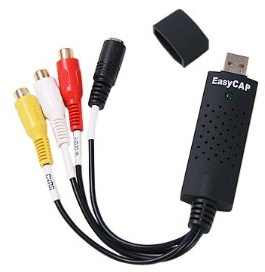
\includegraphics[width=.5\textwidth]{grabber}
 \caption{Der \easycap{}}
\end{figure}

\subsubsection{Videochip \saa}
Der von \emph{Philips Semiconductors} entwicklte \saa{} ist ein 9-Bit-Videoprozessor, der mehrere Eingangssignale verarbeiten und dabei umfangreiche Bildanpassungen wie Helligkeits- und Kontrastanpassung, Farbkorrektur und Rauschreduzierung in Echtzeit durchführen kann \autocite{datasheet:saa7113}.
Fener zeichnet er sich durch eine äußerst kompakte Baugröße und einen niedrigen Energiebedarf aus.

\subsubsection{USB-Gateway-Chip \stk}
Der zweite verbaute Chip ist der von \emph{Syntek Semiconductor} entwickelte USB-Gateway-Chip \stk.
Jener ist zum einen mit dem \saa{} über den von \emph{Philips Semiconductors} entwickelten seriellen Datenbus \iic{} (Inter-Integrated Circuit) und zum anderen über USB~2.0 mit dem Computer verbunden.

\paragraph{\iic}
\iic{} ist ein serieller Datenbus, der entwickelt wurde, um eine einfache, standardisierte Möglichkeit zu besitzen, um zwischen verschiedenen Mikrochips kommunizieren zu können.
Die Kommunikation beschränkt sich hierbei auf Steuerinformationen.
Der Bus ist wie auch USB als Master-Slave-Bus konzipiert, wobei es immer der Master ist, der den Datentransfer beginnt.
In unserem Falle stellt der \stk{} den Master und der \saa{} den Slave dar.

\subsubsection{Zusammenspiel der Chips}
\label{section:zusammenspiel}
Der Computer oder allgemeiner, das Hostsystem kommuniziert immer nur mit dem \stk, nie jedoch mit dem \saa{} direkt.
Sämtliche Steuerinformationen, in der Regel die Manipulation von Registern, die den \stk{} betreffen, werden in USB-Kontrollnachrichten verpackt und an den \stk{} mittels synchronem Transfer gesendet.
Ist es notwendig, Steuerinformationen an den \saa{} zu senden, läuft die Kommunikation folglicherweise über den \stk.
In diesem Falle müssen auch USB-Kontrollnachrichten an den \stk{} gesendet werden, der bei bestimmten Werten in jenen Nachrichten die nötigen Steuerinformationen über \iic{} an den \saa{} weiterleitet.
Die eigentliche Übertragung der Videoinformationen von der Videoquelle durch den \saa{} und dann über den \stk{} zum Hostsystem erfolgt nicht über \iic, da jenes Protokoll mit einer maximalen Datenrate von 3,4\,MBit/s viel zu langsam wäre.
Stattdessen existiert neben dem \iic-Bus eine weitere, 8\,Bit breite Datenverbindung, der \emph{VPO}-Bus.
\begin{figure}[h]
 \centering
 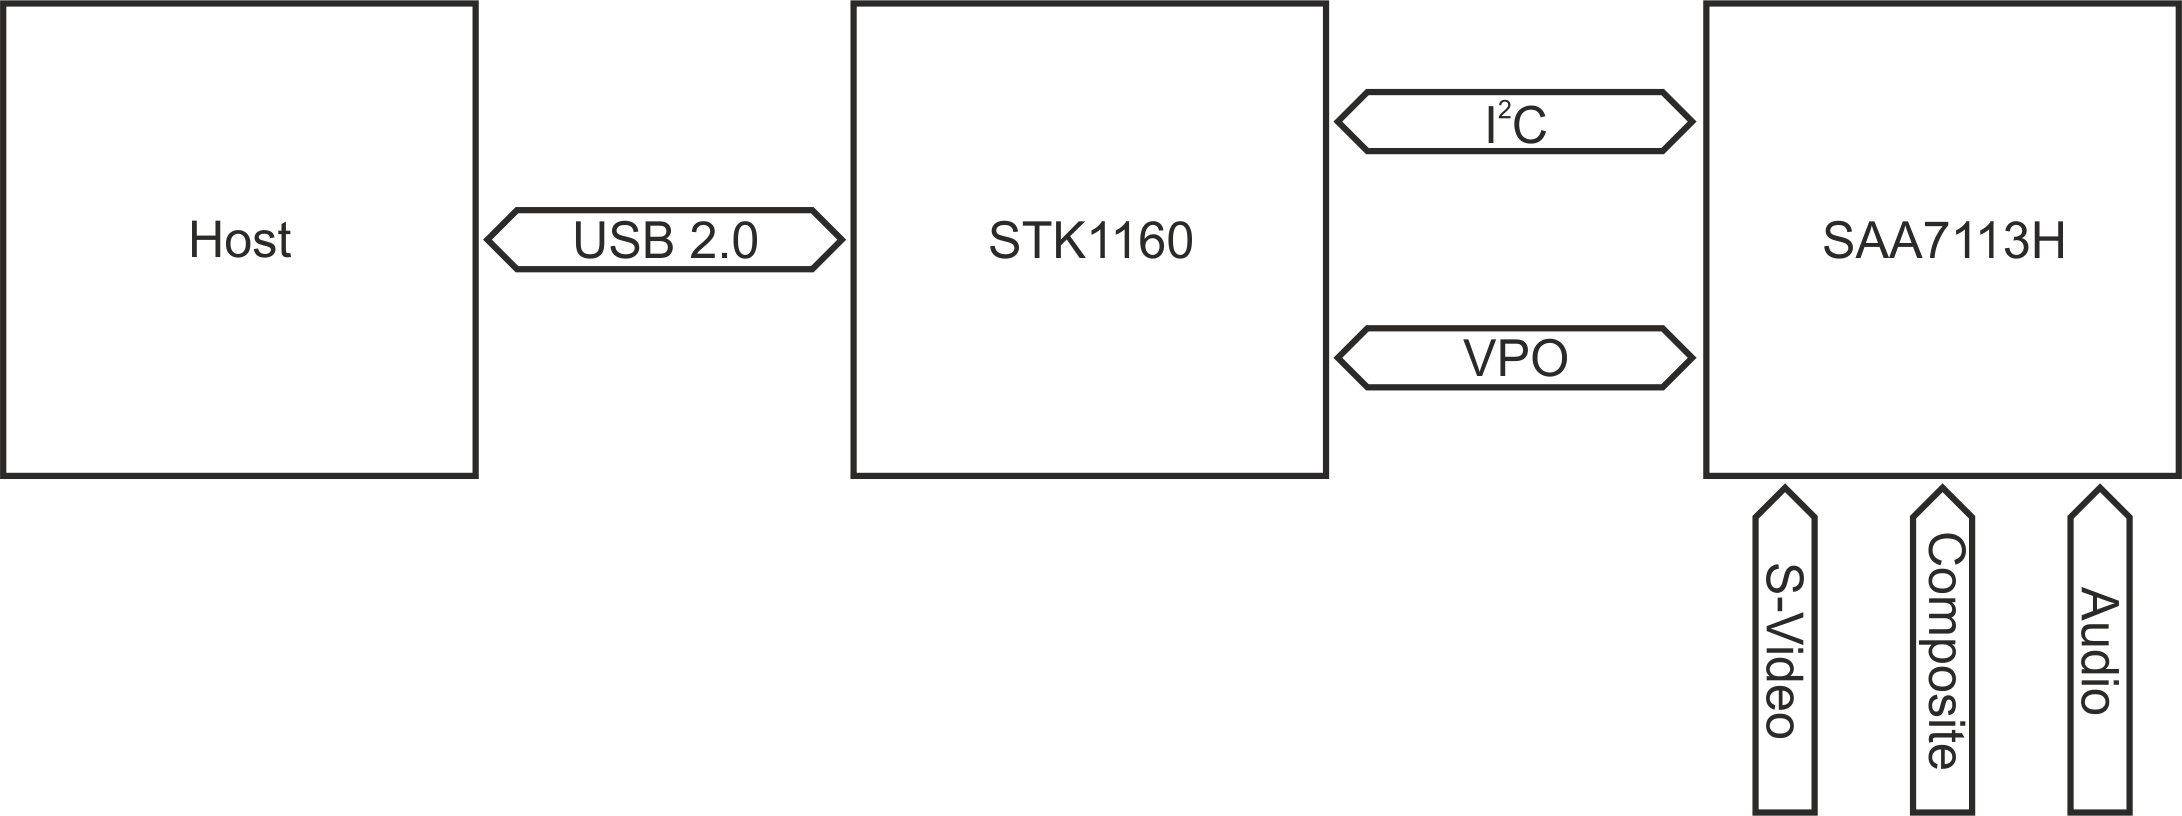
\includegraphics[width=\textwidth]{blockschaltbild}
 \caption{Blockschaltbild des \easycap{}}
\end{figure}

\subsubsection{Übertragung der Videodaten}
Wenn die Videoübertragung beginnen soll, wird ein Register im \saa{} gesetzt.
Die Videodaten werden dann fortlaufend über den \emph{VPO}-Bus in einen Puffer im \stk{} abgelegt.
Werden die Daten vom Hostsystem nicht über isochronen USB-Datentransfer "`abgeholt"', werden sie im Puffer fortlaufend überschrieben.
Liegt jedoch eine leere isochrone USB-Nachricht vor, liest der \stk{} die Videodaten aus dem Puffer aus und schreibt sie in die Nachricht und schickt jene über den USB-Bus zum Hostsystem zurück.
\section{Treiberentwicklung}
\subsection{Anaylse der Linux Treiber}
Für den verwendeten USB-Video-Grabber sind im Linux Kernel bereits zwei 
verschiedene Treiber vorhanden:
\begin{itemize}
 \item Das Modul easycap (nur in Kernel Version 2.6.x)
 \item Die Module stk1160 bzw. saa711x (ab Kernel Version 3.x.y)
\end{itemize}
Da diese Treiber auf ein im Linux Kern 
vorhandenes größeres Video Framework (V4L2) aufsetzten ist ein direktes Portieren der 
entsprechenden Kernel Module nach RIOT nicht ohne weiteres möglich gewesen.
Trotzdem waren die Linux Kernel Module extrem hilfreich bei der Entwicklung
des RIOT Treibers. Unter anderem konnte anhand dieser Module das zusammenspiel
der beiden Chips und die korrekte Ansteuerung selbiger ermittelt werden.
Insbesondere für den Gateway-Chip \stk{} spielten die Linux Treiber eine
besondere Rolle da für diesen Chip kein Datenblatt verfügbar ist. Die Linux 
Treiber waren somit die einzige, uns verfügbare Dokumentation, für diesen Chip. 

\subsubsection{Analyse auf Quellcode-Ebene}
Da es sich bei dem USB-Video-Grabber um einen Clone des weit verbreiteten
easycap-USB-Video-Grabber handelt hatten wir zunächst das easycap genannte Kernel
Modul welches in älteren Linux Versionen vorhanden ist betrachtet. Dieser Treiber
ist in modernern Versionen des Linux Kernel (3.x aufwärts) nicht mehr vorhanden.
Ein Grund hierfür ist die sehr schlechte Code-Qualität und die nahezu
nicht vorhandene Dokumentation dieses Moduls. Wegen der schlechten Lesbarkeits des
Codes war der Informationsgewinn durch das betrachten dieses Codes relativ gering.

In aktuelleren Linux Versionen ist sowohl ein Treiber für den \stk{} (Modulname: stk1160) 
wie auch für den \saa{} (Modulname: saa711x) Chip vorhanden. Diese Treiber sind im wesentlichen 
das Ergebnis eines refactoring des alten easycap Moduls. Der Code dieser Module ist wesentlich 
besser lesbar. Die Dokumentation ist aber auch in diesen Modulen eher mangelhaft. Insbesondere 
lassen sich im Code Kommentare finden die darauf schließen lassen, dass der Autor einige aus easycap übernommenen Teile selber nicht verstanden hat.

Trotz dieser Schwierigkeiten konnten wir anhand der neueren Kernel Module das Grundlegende Zusammenspiel der beiden beteiligten Chips nachvollziehen. Einige Unklarheiten sind jedoch erhalten geblieben. Insbesondere wird in den Modulen stk1160 und saa711x Gebrauch von geschachtelten Makros gemacht und nicht Dokumentierte magische Zahlen verwendet. 

\subsubsection{Anaylse auf funktionaler Ebene}
Unter Linux gibt es ein Kernel Modul (Modulename: usbmon) welches es erlaubt USB-Datentransfers zu beobachten bzw. 
mitzuschneiden. Als Frontend für dieses Modul kann, dass Netzwerkanalyseprogramm wireshark verwendet werden. 
Jedoch kann usbmon keine Datentransfers beobachten welche DMA (Direct Memory Access) nutzen. Da das stk1160 Modul für den 
asynchronen Datentransfer standardmäßig DMA verwendet waren wir gezwungen das Modul zu modifizieren.
Mit dem modifizierten stk1160, usbmon und wireshark war es uns anschließend möglich den Datentransfer zwischen PC
und USB-Video-Grabber im laufenden Betrieb zu beobachten.

\subsubsection{Analyseergebnisse}
Durch die Analyse der Linux Module erschloss sich uns das in \autoref{section:zusammenspiel} dargestellte Zusammenspiel der
beiden Chips. Des weiteren wurde klar, wie die Initialisierung, der Datentransfer, die Deinitialisierung des
USB-Video-Grabbers und die Kommunikation mit dem \saa{} funktioniert:

\paragraph{Kommunikation mit \saa{}:} Der \saa{} Chip kann von PC-Seite aus nur indirekt über den \stk{} Chip angesteuert werden.
Der \stk{} Chip kann angewiesen werden eine \iic{} Nachricht an den \saa{} Chip zu schicken indem der Inhalt der Nachricht in ein
spezielles Register geschrieben wird. Anschließend muss eine Reihe anderer Register mit speziellen Werten beschrieben werden um
die Nachricht abzuschicken. \textbf{!!!!!!!!LISTINGS?!!!!!!!!}

\paragraph{Initialisierung:}
\begin{enumerate}
 \item (\saa{} Chip über \iic{}) Der gewünschte Videostandard und andere Timing Parameter werden konfiguriert.
 \item (\saa{} Chip über \iic{}) Der \saa{} wird angewiesen Videodaten an den \stk{} weiterzuleiten.
 \item (\stk{} Chip) Der Chip wird angewiesen isochrone USB-Anfragen zu beantworten.
\end{enumerate}

\paragraph{Datentransfer:} Ist die Initialisierung abgeschlossen können vom PC isochrone USB Pakete an den USB-Video-Grabber
geschickt werden. Jedoch ist darauf zu achten, dass auf dem Host-Controller genügend Bandbreite für den Datentransfer reserviert wird
(vgl. \emph{Alternate Setting}). Im wesentlichen funktioniert der Datentransfer wie folgt:
\begin{enumerate}
 \item Leere Pakete (URBs) werden von dem PC an den \stk{} geschickt.
 \item Der \stk{} befüllt diese Pakete mit den Videodaten und sendet diese nach einer unbekannten Zeitspanne zurück an den Sender.
 \item Der Treiber hat einen asynchronen handler welcher beim eintreffen eines Antwortpaketes folgendermaßen agiert:
 \begin{enumerate}
  \item Die Integrität der Daten wird geprüft (anhand einer CRC16 Prüfsumme).
  \item Die Daten werden in einen Puffer geschrieben.
  \item Ein leeres Paket wird erzeugt und wieder an den \stk{} geschickt. 
 \end{enumerate}
\end{enumerate}
Die Fehlerbehandlung haben wir im Sinne der Übersichtlichkeit nicht dargestellt.

\paragraph{Deinitialisierung:}
\begin{enumerate}
 \item 
\end{enumerate}


\subsection{Aufbau und Funktionsweise des RIOT Treibers}


\subsection{Vorgehen bei der Implementierung}

\subsection{Probleme und Herausforderungen}


\section{Abschlussbetrachtung}

\subsection{Veränderung der Projektvorgaben}
Die übersprüngliche Projektbeschreibung sah vor, dass ein Gerätetreiber für eine Kamera entwickelt werden sollte, dabei war allerdings nicht näher spezifiert, wie diese Kamera geartet sein sollte.
Nachdem sich herausstellte, dass die Kamera für das Softwareprojekt nicht verfügbar sein würde, veränderte sich das Projekt dahingehend, dass von jenem Zeitpunkt an ein Gerätetreiber für einen USB-Video-Grabber entwickelt werden sollte.

Die Plattform, für welche der Treiber entwickelt werden sollte, war hierbei das Board \emph{MSBA2}, für welches eine Portierung von RIOT existiert.
Hier tat sich bereits am Anfang die Frage auf, ob das \emph{MSBA2} genug Rechenleistung und Speicher bieten könnte, um entsprechende Puffer zu allozieren; wenig später beantwortete sich jene Frage nach der Einarbeitung in die Programmierung des \emph{MSBA2} bei der Analyse des existierenden Linux-Treibers von selbst.
Es ergab sich, dass das \emph{MSBA2} mit einem Arbeitsspeicher von nur 98\,KiB nicht für die Verarbeitung der Videodaten geeignet war.

Anschließend wurde mit dem \emph{BeagleBone}, einem günstigen Computer auf einer Platine, eine neue Hardwareplattform eingeführt, die wesentlich mehr Rechenleistung und Arbeitsspeicher bot, jedoch änderte sich diese Vorgabe bereits wieder in der nächste Woche.

Die finale Plattform war schließlich der \emph{native port} von RIOT (siehe \autoref{section:native_port}), der praktisch alle Beschränkungen von Rechenleistung und Arbeitsspeicher aufhob und die Möglichkeit, auf eine existierende USB-Funktionalität zurückgreifen zu können, eröffnete.

\subsection{Diskussion des Ergebnisses}
Das Ergebnis dieses Softwareprojektes ist im Grunde genommen ein unfertiger Gerätetreiber, der es zulässt, den \stk{} und den \saa{} zu konfigurieren und welcher tatsächlich einen Videostream bereitstellt, jedoch sind die Videodaten bis zum heutigen Zeitpunkt noch relativ nutzlos, da sie nur bedigt etwas mit der Realität zu tun haben.
\footnote{Helligkeitsunterschiede waren zu erkennen}
Der Hauptgrund dafür ist die Tatsache, dass der verwendete USB-Video-Grabber sowie die Verwendung des \emph{native port} erst gemessen an der Gesamtdauer des Softwareprojektes sehr spät feststand.
Der damit einhergehende effektive Zeitverlust ließ uns zum Ende des Projektes hin nicht mehr die Möglichkeit, die Videodaten einer umfangreichen Analyse zu unterziehen sowie die fehlende Funktionalität, was besonders die Kontrolle des \saa{} betrifft, zu implementieren.

\subsection{Ausblick}
Bis zum produktiven Einsatz des Treibers ist es noch ein relativ weiter Weg, da es noch Baustellen an verschiedenen Stellen gibt:
Es müssen diverse Funktionen des \saa, zum Beispiel Bildverarbeitungen wie Hellkeits- und Kontrastanpassungen oder die Frameratesteuererung, konfigurierbar gemacht werden.
Dazu ist es nötig, das Datenblatt des \saa{} zu studieren und auch den Linuxtreiber weiter zu betrachten.
Ferner ist auch notwendig, die empfangenen Daten zu validieren und an der Interpretation derjenigen zu arbeiten, um überhaupt ein brauchbares Bild zu erhalten.
Zum Abschluss sei noch angemerkt, dass für RIOT noch ein USB-Stack notwendig ist, um gegebenenfalls \libusb{} zu protieren oder gleich die fiktive native USB-Funktionalität von RIOT zu nutzen.

\subsection{Reflexion}
Dieses Softwareprojekt war durch und durch eine interessante Herausforderung und gleichwohl eine hervorragende Möglichkeit, Kenntnisse in vielen Bereichen zu erhalten:
\begin{itemize}
 \item Funktionsweise des USB-Protokolles
 \item Programmierung eines Gerätetreibers
 \item Verwendung von vielen Entwicklungswerkzeugen wie \emph{vim}, \emph{ctags}, \emph{gcc}, \emph{gdb}, \emph{git} und vielen anderen mehr ...
 \item Beflügelung durch Teilerfolge und Demotivation durch Rückschläge
\end{itemize}
Alles in allem ist es eine wertvolle Erfahrung, solch ein Softwareprojekt durchzuführen.
Wir lernten, Arbeit aufzuteilen, zu strukturieren, diese Zweige wieder zusammenzuführen.

Ein bisschen schade ist es aus unserer Sicht am Ende doch, kein Richtiges Bild bekommen zu haben, aber sicherlich wird irgendwann auf Basis dieses Softwareprojektes etwas weiterenwickelt.

\newpage
\printbibliography

\end{document}
